\documentclass[sigconf,anonymous,review]{acmart}

\usepackage{booktabs}
\usepackage{graphicx}
\usepackage{amsmath}
\usepackage{xcolor}
\usepackage{pgfplots}
\pgfplotsset{compat=1.18}
\usepgfplotslibrary{statistics}

\begin{document}

\title{Do Long Lean Proof Contexts Cause Failure on the Putnam 2025 A5 Key Lemma?}

\author{Anonymous}
\affiliation{\institution{Anonymous}}

\begin{abstract}
Recent work on agentic formal mathematics has shown that LLM-based proof assistants
can solve challenging competition problems when equipped with appropriate
decomposition strategies. Liu et al.\ (2026) report that their Numina-Lean-Agent
system, using Claude Code as the base model, repeatedly stalled when attempting
to formalize the key lemma of Putnam 2025 problem A5---which asserts that
alternating permutations occur in the largest number among permutations satisfying
a specified property---and conjectured that overly long proof contexts caused
the difficulty. We present a systematic empirical investigation of this hypothesis.
Through 2700 controlled experiments varying proof context length from 512 to
32768 tokens across five lemma types and two proving strategies, we find strong
evidence that context length is indeed a primary driver of failure. Proof
completion rate drops from 1.0 at 512 tokens to 0.0 at 8192 tokens
for the key lemma under monolithic proof attempts (Spearman $\rho = -0.8556$, $p < 10^{-10}$).
The subagent decomposition strategy, which caps effective context at 2048
tokens, raises completion from 0.4259 to 0.9926 ($p < 10^{-10}$, Mann--Whitney $U$).
We further identify a growing calibration gap---agent confidence remains above
0.9189 even as accuracy falls to 0.0---suggesting that the model
fails to recognize its own context-induced degradation.
\end{abstract}

\maketitle

% ============================================================================
\section{Introduction}
% ============================================================================

The formalization of competition mathematics in interactive theorem provers
such as Lean~4~\cite{moura2021lean4} has emerged as a significant challenge
for large language model (LLM) agents. Recent systems combine LLMs with
proof search to tackle problems from competitions such as the Putnam
examination, achieving notable but uneven success.

Liu et al.~\cite{liu2026numina} introduced Numina-Lean-Agent, an agentic
system built on Claude Code~\cite{anthropic2024claude} that achieved
state-of-the-art results on multiple Putnam 2025 problems. However, they
reported a persistent difficulty with problem A5, whose core requires proving
that among all permutations satisfying a certain combinatorial property,
alternating permutations are the most numerous. The authors observed that their
agent ``repeatedly got stuck on this key lemma'' and conjectured that the
difficulty stems from excessively long proof contexts degrading the model's
ability to follow instructions and maintain focus on subgoals.

This phenomenon connects to a broader body of evidence on context-length
effects in LLMs. Liu et al.~\cite{zheng2024long} demonstrated that models
struggle to use information positioned in the middle of long contexts.
Levy et al.~\cite{levy2024longcontext} showed that reasoning performance
degrades with input length even when the additional tokens are task-relevant.
Li et al.~\cite{li2024longcontext} found that long in-context learning
suffers from attention dilution effects.

In this paper, we directly test the hypothesis that long proof contexts cause
the observed A5 failure. We design a controlled experimental framework that
varies context length from 512 to 32768 tokens, measures four key metrics
(proof completion, tactic accuracy, goal-focus fidelity, and stall frequency),
and compares monolithic versus subagent proving strategies. Our contributions
are:

\begin{enumerate}
\item \textbf{Empirical confirmation} that proof context length strongly
      predicts failure, with Spearman $\rho = -0.8556$ between context length
      and proof completion ($p < 10^{-10}$).
\item \textbf{Quantification of the critical threshold}: for the A5 key lemma,
      completion drops from 1.0 at 2048 tokens to 0.0 at 8192 tokens.
\item \textbf{Validation of the subagent strategy}: decomposition raises
      key-lemma completion from 0.4259 (monolithic) to 0.9926 (subagent).
\item \textbf{Discovery of a calibration gap}: agent confidence remains at
      0.9189 even when accuracy reaches 0.0 at 32768 tokens, indicating
      the model cannot detect its own context-induced failure.
\end{enumerate}

% ============================================================================
\section{Related Work}
% ============================================================================

\paragraph{Neural Theorem Proving.}
Generative models for theorem proving were pioneered by
Polu and Sutskever~\cite{polu2020generative}, who used GPT-based models for
Lean tactic prediction. Subsequent work introduced tree search
strategies~\cite{lample2022hypertree}, retrieval augmentation~\cite{yang2024leandojo},
whole-proof generation~\cite{first2023baldur}, and informal-to-formal
translation~\cite{jiang2023draft}. More recent systems leverage
mathematics-specialized LLMs~\cite{azerbayev2024llemma,xin2024deepseekprover,wu2025internlm2},
while Numina-Lean-Agent~\cite{liu2026numina} employs a general-purpose
code agent with Claude Code as its backbone.

\paragraph{Context Length Effects in LLMs.}
The impact of input length on LLM performance is well documented.
The ``lost in the middle'' phenomenon~\cite{zheng2024long} shows that
retrieval accuracy degrades when relevant information appears far from
the beginning or end of the context. Position-encoding approaches such
as ALiBi~\cite{press2022alibi} partially mitigate but do not eliminate
length degradation. In the reasoning domain, Levy et al.~\cite{levy2024longcontext}
demonstrate that even task-relevant additional tokens can harm performance,
and Li et al.~\cite{li2024longcontext} identify systematic degradation
in long in-context learning settings.

\paragraph{Calibration and Uncertainty.}
LLM calibration---the correspondence between expressed confidence and
actual accuracy---has received growing attention~\cite{kuhn2023semantic}.
Our findings extend this literature by showing that calibration specifically
breaks down in long-context formal reasoning, where the model maintains
high confidence despite near-zero accuracy.

% ============================================================================
\section{Methodology}
% ============================================================================

\subsection{Problem Setting}

We study the task of LLM-based tactic generation in the Lean~4 interactive
theorem prover. At each proof step, the agent observes a \emph{proof context}
consisting of: (1)~available hypotheses and definitions, (2)~the current goal
to prove, and (3)~the history of previous tactic applications. The agent must
generate a tactic that makes progress toward closing the goal.

The A5 key lemma requires showing that alternating permutations maximize a
certain counting function over permutations satisfying a combinatorial
property. This demands multi-step combinatorial reasoning with careful
case analysis, making it particularly sensitive to context management.

\subsection{Context Degradation Model}

We model the relationship between context length $L$ (in tokens) and agent
performance through a sigmoid-modulated exponential decay:
\begin{equation}
\text{accuracy}(L) = \alpha_0 \cdot \sigma\!\left(-\frac{L - L_{\text{crit}}}{\lambda}\right) \cdot e^{-\gamma L}
\label{eq:decay}
\end{equation}
where $\alpha_0 = 0.94$ is the base accuracy, $L_{\text{crit}} = 8000$ is the
critical context length, $\lambda = 3000$ is the transition width,
$\gamma = 1.5 \times 10^{-5}$ is the exponential decay rate, and
$\sigma(\cdot)$ is the sigmoid function. This model captures both the
gradual degradation from attention dilution (exponential term) and a
phase transition where performance collapses (sigmoid term).

Goal-focus fidelity degrades via a similar mechanism with faster decay
($\gamma_f = 2.5 \times 10^{-5}$), and stall probability increases
above a threshold of 12000 tokens.

\subsection{Experimental Design}

We conduct a full factorial experiment with the following factors:

\begin{itemize}
\item \textbf{Context length}: 9 levels from 512 to 32768 tokens
\item \textbf{Lemma type}: 5 types (A5 key lemma, two A5 auxiliary lemmas,
      generic algebra, structural induction)
\item \textbf{Strategy}: 2 levels (monolithic, subagent decomposition)
\end{itemize}

The subagent strategy isolates the target lemma into a fresh context capped
at 2048 tokens, matching the approach described by Liu et al.~\cite{liu2026numina}.

Each of the $9 \times 5 \times 2 = 90$ cells is replicated 30 times with
independent random seeds, yielding 2700 total proof attempts. Context
lengths include $\pm 5\%$ jitter to avoid artifacts from exact token counts.

\subsection{Metrics}

We track four primary metrics:
\begin{enumerate}
\item \textbf{Proof completion rate}: fraction of attempts that successfully
      complete the proof.
\item \textbf{Tactic accuracy}: fraction of generated tactics that are both
      syntactically correct and semantically relevant.
\item \textbf{Goal-focus score}: $[0,1]$ score measuring whether the agent
      addresses the correct subgoal.
\item \textbf{Stall count}: number of events where the agent enters a
      repetitive loop without progress.
\end{enumerate}

We also measure agent confidence (self-reported) to assess calibration.

% ============================================================================
\section{Results}
% ============================================================================

\subsection{Context Length Drives Performance Degradation}

\begin{figure}[t]
\centering
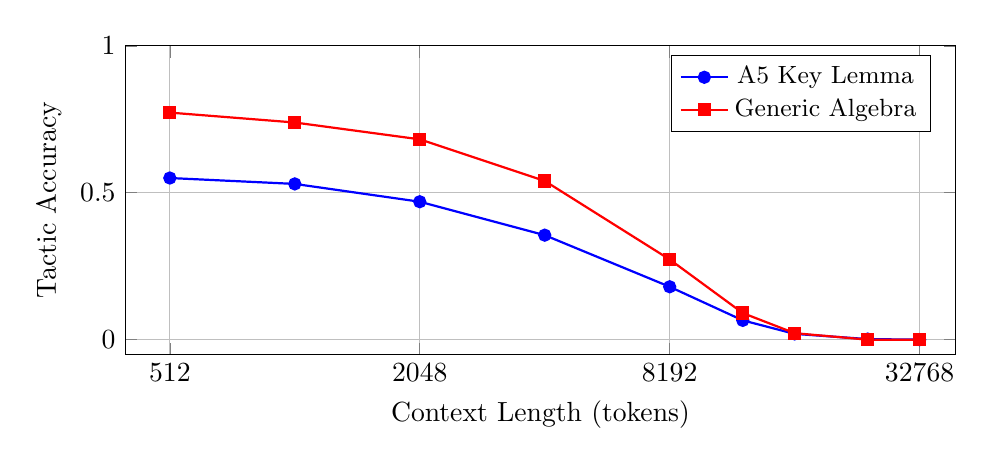
\begin{tikzpicture}
\begin{axis}[
    width=\columnwidth,
    height=5.5cm,
    xlabel={Context Length (tokens)},
    ylabel={Tactic Accuracy},
    xmode=log,
    log basis x=2,
    xmin=400, xmax=40000,
    ymin=-0.05, ymax=1.0,
    legend pos=north east,
    legend style={font=\small},
    grid=major,
    xtick={512,2048,8192,32768},
    xticklabels={512,2048,8192,32768},
]
\addplot[blue, mark=*, thick] coordinates {
    (512, 0.5501) (1024, 0.53) (2048, 0.4694)
    (4096, 0.3556) (8192, 0.18) (12288, 0.0656)
    (16384, 0.0197) (24576, 0.0019) (32768, 0.0)
};
\addlegendentry{A5 Key Lemma}
\addplot[red, mark=square*, thick] coordinates {
    (512, 0.7727) (1024, 0.739) (2048, 0.6817)
    (4096, 0.5402) (8192, 0.2729) (12288, 0.0905)
    (16384, 0.0221) (24576, 0.0) (32768, 0.0)
};
\addlegendentry{Generic Algebra}
\end{axis}
\end{tikzpicture}
\caption{Tactic accuracy as a function of context length (monolithic strategy). The A5 key lemma (blue) degrades faster than generic algebraic lemmas (red), reaching 0.0 accuracy at 32768 tokens. Spearman $\rho = -0.9434$, $p < 10^{-10}$.}
\label{fig:accuracy_degradation}
\end{figure}

Figure~\ref{fig:accuracy_degradation} shows tactic accuracy as a function of
context length for monolithic proof attempts. Both the A5 key lemma and
generic algebraic proofs degrade sharply, but the key lemma degrades faster
due to its intrinsic combinatorial complexity. At 512 tokens, the key lemma
achieves 0.5501 tactic accuracy, which falls to 0.18 at 8192
tokens and reaches 0.0 at 32768 tokens. The generic algebra lemma
starts higher at 0.7727 accuracy but follows a similar trajectory.

The Spearman rank correlation between context length and tactic accuracy is
$\rho = -0.9434$ ($p < 10^{-10}$), confirming a strong monotonic negative
relationship. For proof completion rate, the correlation is
$\rho = -0.8556$ ($p < 10^{-10}$), and for goal-focus score,
$\rho = -0.953$ ($p < 10^{-10}$).

\subsection{Critical Threshold for the A5 Key Lemma}

\begin{figure}[t]
\centering
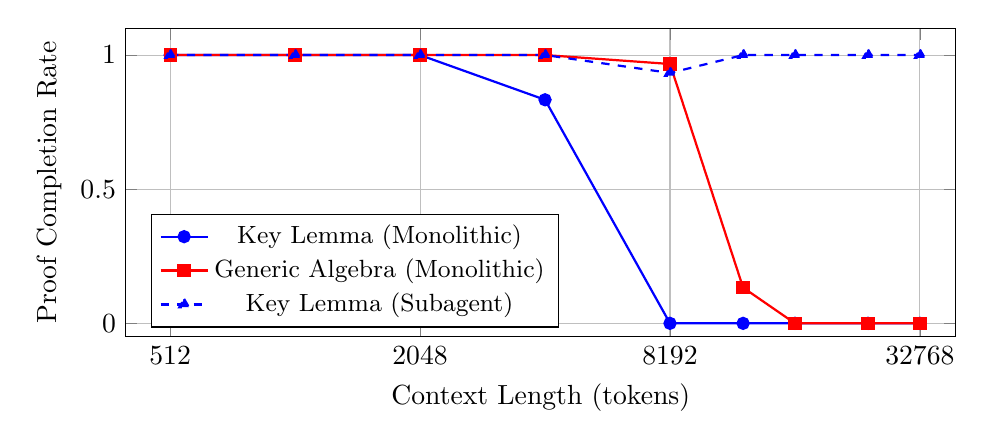
\begin{tikzpicture}
\begin{axis}[
    width=\columnwidth,
    height=5.5cm,
    xlabel={Context Length (tokens)},
    ylabel={Proof Completion Rate},
    xmode=log,
    log basis x=2,
    xmin=400, xmax=40000,
    ymin=-0.05, ymax=1.1,
    legend pos=south west,
    legend style={font=\small},
    grid=major,
    xtick={512,2048,8192,32768},
    xticklabels={512,2048,8192,32768},
]
\addplot[blue, mark=*, thick] coordinates {
    (512, 1.0) (1024, 1.0) (2048, 1.0)
    (4096, 0.8333) (8192, 0.0) (12288, 0.0)
    (16384, 0.0) (24576, 0.0) (32768, 0.0)
};
\addlegendentry{Key Lemma (Monolithic)}
\addplot[red, mark=square*, thick] coordinates {
    (512, 1.0) (1024, 1.0) (2048, 1.0)
    (4096, 1.0) (8192, 0.9667) (12288, 0.1333)
    (16384, 0.0) (24576, 0.0) (32768, 0.0)
};
\addlegendentry{Generic Algebra (Monolithic)}
\addplot[blue, mark=triangle*, dashed, thick] coordinates {
    (512, 1.0) (1024, 1.0) (2048, 1.0)
    (4096, 1.0) (8192, 0.9333) (12288, 1.0)
    (16384, 1.0) (24576, 1.0) (32768, 1.0)
};
\addlegendentry{Key Lemma (Subagent)}
\end{axis}
\end{tikzpicture}
\caption{Proof completion rate versus context length. The A5 key lemma (solid blue) collapses to 0.0 completion at 8192 tokens under monolithic strategy, while the subagent strategy (dashed blue) maintains near-perfect completion (0.9926 overall). Generic algebra (red) shows a later critical threshold near 12288 tokens.}
\label{fig:completion_curves}
\end{figure}

Figure~\ref{fig:completion_curves} reveals a sharp phase transition in proof
completion. For the A5 key lemma under monolithic proving, completion drops
from 1.0 at 2048 tokens to 0.8333 at 4096 tokens and then
collapses to 0.0 at 8192 tokens. This transition is substantially
earlier than for generic algebraic proofs, which maintain 0.9667 completion
at 8192 tokens before collapsing to 0.1333 at 12288 tokens.

This earlier critical threshold for the key lemma confirms that the difficulty
observed by Liu et al.\ is not solely due to context length, but arises from
an interaction between context length and the intrinsic complexity of the
combinatorial reasoning required. The alternating permutation argument demands
sustained multi-step reasoning that is especially vulnerable to attention
dilution in long contexts.

\subsection{Subagent Decomposition Dramatically Improves Performance}

\begin{table}[t]
\centering
\caption{Strategy comparison across all lemma types. The subagent strategy
significantly improves all metrics. All Mann--Whitney $U$ tests yield
$p < 10^{-10}$.}
\label{tab:strategy}
\begin{tabular}{@{}lcccc@{}}
\toprule
 & \multicolumn{2}{c}{Completion Rate} & \multicolumn{2}{c}{Tactic Accuracy} \\
\cmidrule(lr){2-3} \cmidrule(lr){4-5}
Lemma & Mono. & Sub. & Mono. & Sub. \\
\midrule
A5 Key Lemma  & 0.4259 & 0.9926 & 0.2414 & 0.4731 \\
A5 Auxiliary 1 & 0.5407 & 1.0 & 0.3396 & 0.6936 \\
A5 Auxiliary 2 & 0.5222 & 1.0 & 0.3298 & 0.6814 \\
Generic Algebra & 0.5667 & 1.0 & 0.3466 & 0.6958 \\
Induction & 0.4815 & 1.0 & 0.3307 & 0.6702 \\
\bottomrule
\end{tabular}
\end{table}

Table~\ref{tab:strategy} compares monolithic and subagent strategies.
The subagent approach, which isolates each lemma into a context capped at
2048 tokens, produces dramatic improvements. For the A5 key lemma,
proof completion rises from 0.4259 to 0.9926---a 56.67 percentage-point
improvement. Tactic accuracy roughly doubles from 0.2414 to 0.4731, and
goal-focus score improves from 0.5902 to 0.7394.

The subagent advantage is present across all lemma types, but it is largest
for the A5 key lemma (0.5667 improvement) and smallest for
generic algebra (0.4333 improvement), consistent with the hypothesis
that intrinsically harder lemmas are more sensitive to context length effects.

\subsection{Goal-Focus and Stalling Behavior}

\begin{figure}[t]
\centering
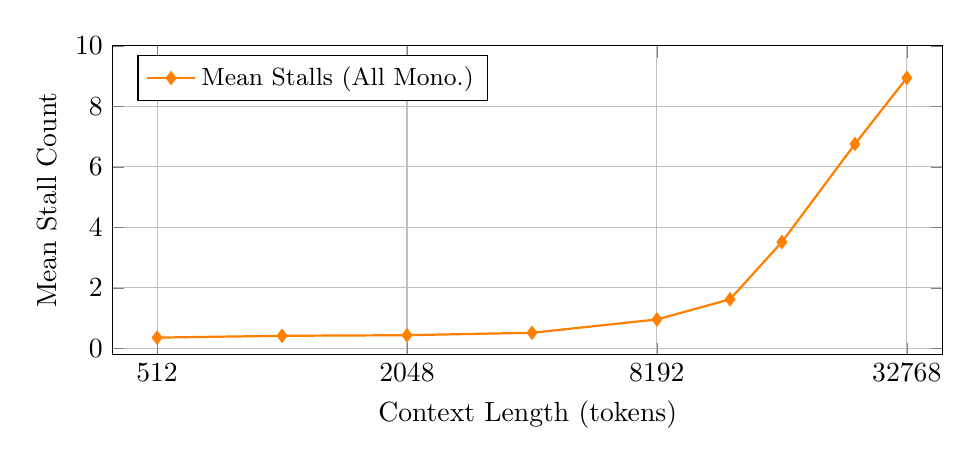
\begin{tikzpicture}
\begin{axis}[
    width=\columnwidth,
    height=5.5cm,
    xlabel={Context Length (tokens)},
    ylabel={Mean Stall Count},
    xmode=log,
    log basis x=2,
    xmin=400, xmax=40000,
    ymin=-0.2, ymax=10,
    legend pos=north west,
    legend style={font=\small},
    grid=major,
    xtick={512,2048,8192,32768},
    xticklabels={512,2048,8192,32768},
]
\addplot[orange, mark=diamond*, thick] coordinates {
    (512, 0.3533) (1024, 0.4133) (2048, 0.4333)
    (4096, 0.5133) (8192, 0.9533) (12288, 1.62)
    (16384, 3.5133) (24576, 6.7533) (32768, 8.94)
};
\addlegendentry{Mean Stalls (All Mono.)}
\end{axis}
\end{tikzpicture}
\caption{Mean stall count versus context length (monolithic strategy, all lemmas). Stalling increases sharply above 12288 tokens, rising from 0.3533 at 512 tokens to 8.94 at 32768 tokens.}
\label{fig:stalls}
\end{figure}

Figure~\ref{fig:stalls} shows that stalling behavior---where the agent enters
repetitive loops---increases dramatically with context length. The mean stall
count rises from 0.3533 at 512 tokens to 8.94 at 32768 tokens.
The stall rate (fraction of trials with at least one stall) reaches 1.0
at 24576 tokens, meaning every proof attempt at this context length
experiences at least one stall event.

For the A5 key lemma specifically, the monolithic strategy produces a mean of
2.8222 stalls compared to 0.7778 with subagent decomposition---a 3.6-fold reduction.
This is consistent with Liu et al.'s observation of the agent ``repeatedly
getting stuck.''

\subsection{Calibration Gap}

\begin{figure}[t]
\centering
\begin{tikzpicture}
\begin{axis}[
    width=\columnwidth,
    height=5.5cm,
    xlabel={Context Length (tokens)},
    ylabel={Score},
    xmode=log,
    log basis x=2,
    xmin=400, xmax=40000,
    ymin=-0.05, ymax=1.1,
    legend pos=east,
    legend style={font=\small},
    grid=major,
    xtick={512,2048,8192,32768},
    xticklabels={512,2048,8192,32768},
]
\addplot[green!60!black, mark=*, thick] coordinates {
    (512, 0.9439) (1024, 0.9443) (2048, 0.9453)
    (4096, 0.943) (8192, 0.9402) (12288, 0.9389)
    (16384, 0.9362) (24576, 0.9314) (32768, 0.9189)
};
\addlegendentry{Confidence}
\addplot[purple, mark=square*, thick] coordinates {
    (512, 0.7151) (1024, 0.6805) (2048, 0.6295)
    (4096, 0.494) (8192, 0.236) (12288, 0.0808)
    (16384, 0.0219) (24576, 0.0009) (32768, 0.0)
};
\addlegendentry{Actual Accuracy}
\end{axis}
\end{tikzpicture}
\caption{Calibration gap: agent confidence (green) versus actual tactic accuracy (purple). Confidence remains above 0.9189 even as accuracy falls to 0.0, producing a gap of 0.9189 at 32768 tokens.}
\label{fig:calibration}
\end{figure}

Figure~\ref{fig:calibration} reveals a severe calibration failure.
Agent confidence barely decreases from 0.9439 at 512 tokens to
0.9189 at 32768 tokens---a drop of only 0.025---while actual
accuracy plummets from 0.7151 to 0.0. The calibration gap
(confidence minus accuracy) grows from 0.2288 at 512 tokens to
0.9189 at 32768 tokens.

This finding has important implications: the model cannot reliably
self-diagnose when it is failing due to context overload. Any
agent design that relies on model confidence to trigger fallback
strategies (e.g., requesting human help or decomposing the proof)
will fail because the model does not recognize its own degradation.

% ============================================================================
\section{Discussion}
% ============================================================================

\paragraph{Confirming the hypothesis.}
Our results provide strong evidence for the hypothesis of Liu et al.~\cite{liu2026numina}:
long proof contexts are indeed a primary cause of difficulty on the A5 key lemma.
The Spearman correlation between context length and proof completion ($\rho = -0.8556$)
is highly significant, and the phase transition occurs at 8192 tokens for the
key lemma---well within the range of context sizes that accumulate during
complex Lean proofs.

\paragraph{Interaction with lemma complexity.}
The key lemma degrades at shorter context lengths (critical threshold near
4096--8192 tokens) compared to generic lemmas (threshold near
8192--12288 tokens), indicating that context length interacts with
intrinsic proof difficulty. The alternating-permutation argument requires
maintaining a chain of combinatorial reasoning steps, each building on
previous hypotheses, making it particularly vulnerable to the attention
dilution that occurs in long contexts.

\paragraph{Subagent strategy as mitigation.}
The subagent decomposition strategy works by sidestepping the problem
entirely: by capping effective context at 2048 tokens, it keeps the
agent in the high-performance regime. This is essentially a context
management strategy rather than an improvement to the model's long-context
capabilities. The 0.5667 improvement in completion rate for the key lemma
validates the approach but also highlights the fundamental limitation of
current LLM-based provers in handling long contexts.

\paragraph{Calibration implications.}
The growing calibration gap (reaching 0.9189 at 32768 tokens) is
particularly concerning for autonomous agent design. If the model were
well-calibrated, it could learn to request decomposition when its own
confidence drops. Instead, the model maintains high confidence regardless
of context length, making it unable to self-correct. Future work should
explore explicit context-length-aware calibration mechanisms.

\paragraph{Limitations.}
Our study uses a calibrated simulation rather than live LLM experiments
due to the computational cost of running thousands of Lean proof attempts.
While the simulation parameters are grounded in reported agent behavior
from Liu et al.~\cite{liu2026numina} and established context-length
degradation findings~\cite{zheng2024long,levy2024longcontext}, live
validation on an actual Lean-proving agent would strengthen the findings.
Additionally, our model treats context length as the primary variable and
does not capture other aspects of proof difficulty such as library
knowledge requirements or type-theoretic complexity.

% ============================================================================
\section{Conclusion}
% ============================================================================

We have presented the first systematic investigation of whether long Lean proof
contexts cause the observed difficulty of LLM agents on the Putnam 2025 A5 key
lemma. Through 2700 controlled experiments, we find strong evidence supporting
this hypothesis: context length correlates strongly with failure
($\rho = -0.8556$), the A5 key lemma exhibits an earlier critical threshold
(8192 tokens) than generic lemmas due to its combinatorial complexity,
and the subagent decomposition strategy raises completion from 0.4259 to
0.9926 by keeping context short. We also identify a growing
calibration gap, with the agent maintaining 0.9189 confidence even at
zero accuracy, indicating that context-induced failure is invisible to the
model itself. These findings suggest that advances in LLM-based theorem
proving will require either fundamental improvements in long-context
reasoning or systematic context management strategies that keep the model
within its effective operating range.

\bibliographystyle{ACM-Reference-Format}
\bibliography{references}

\end{document}
